%% ------------------------------------------------------------------------- %%
\chapter{Ajuste dos hiper-parâmetros e normalização em lote}
\label{cap:ajuste-hiper-parametros-cnn}

Neste capítulo apresentamos os resultados dos ajustes dos hiper-parâmetros e da normalização em lote feita nas arquiteturas convolucional e \textbf{Unif}. O intuito destes ajustes é obter um modelo mais robusto e evitar o \textit{overfitting}.

\section{Ajuste dos hiper-parâmetros da rede convolucional}
\label{sec:ajuste-hiper-parametros-cnn}

A rede convolucional exige alguns hiper-parâmetros que devem ser informados durante o treinamento. O tamanho da entrada, conforme citado no capítulo~\ref{cap:experimento}, foi fixado em 150. Caso as palavras tenham tamanho menor, o vetor é preenchido com valores $0$ ao final. Outros três parâmetros exigidos pela rede convolucional são: filtros, kernel e stride.

O parâmetro kernel define o tamanho da janela de operação de convolução. No nosso caso, que estamos utilizando a operação de convolução de 1 dimensão, Conv1D \todo{adicionar na explicação}, o kernel define os n-grams a ser extraídos do vetor de entrada. 
O parâmetro filtros define a dimensão de saída da operação de convolução. Este parâmetro indica a quantidade de filtros no resultado da operação de convolução. Cada filtro tenta extrair uma característica diferente do vetor de entrada.

O parâmetro stride define a quantidade de posições de deslocamento do filtro. O parâmetro stride foi fixado em 1. Neste caso, o filtro desloca-se por todas as posições do vetor de entrada de uma em uma posição.

Com relação a quantidade de filtros e o tamanho do kernel, fizemos alguns testes utilizando como base os experimentos feitos por \cite{feng-2015} e \cite{tan-lstm-qa}. Tanto \cite{feng-2015} quanto \cite{tan-lstm-qa} utilizaram o parâmetro filtros com o valor entre 1000 e 4000. Conforme citado no capítulo~\ref{cap:experimento}, a média de palavras na base disponibilizada por \cite{feng-2015} é XXX \todo{coletar a quantidade palavras do insurance}, enquanto nos dados que estamos utilizando é YYYY. 

\subsection{Filtros}

Inicialmente, analisamos o comportamento da rede convolucional utilizando diferentes quantidades de filtros. Nas figuras a seguir, exibimos um gráfico de comparação do valor do erro durante o treinamento em comparação com o erro durante a validação. Foram analisadas as seguintes quantidades de filtros: 50, 100, 200, 500, 1000, 2000, 4000. Inicialmente, utilizamos o kernel com o valor 2, valor recomendado por \cite{tan-lstm-qa}.


\begin{figure}[h]
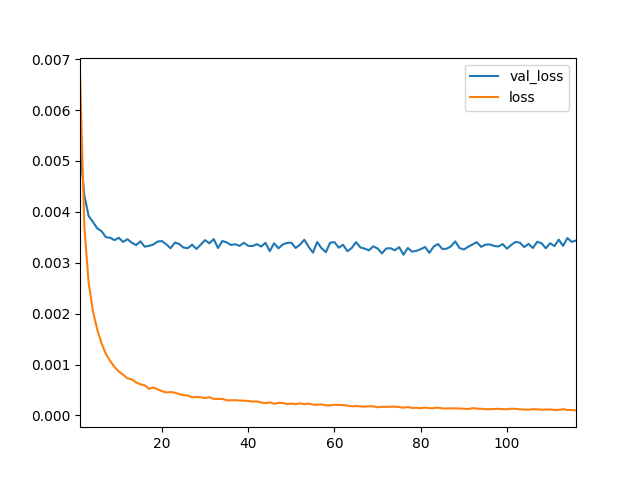
\includegraphics[width=8cm]{figuras/ape-ajustes-hiper-parametros/training-cnn-1000-k-2.png}
\caption{Gráfico do treinamento da rede convolucional na recuperação de trecho de código-fonte. Este gráfico apresenta um comparativo do erro no conjunto de validação em comparação com o erro no conjunto de treinamento. O treinamento é interrompido quando o erro no conjunto de treinamento for ´menor que $1x10^(-4)$ ou ultrapassar 500 épocas.}
\label{fig:ape-cnn-1000-k-2}
\end{figure}


\todo{adicionar os graficos. Rodar os testes de 50, 100, 200, 500 com filtros de tamanho 2}

\subsection{Kernel}

Conforme exibido no capítulo Arquitetura \todo{adicionar referência a arquitetura}, o kernel define na rede convolucional de 1 dimensão, o n-grams a serem extraídos. Durante o treinamento, analisamos diferentes valores para o kernel. Verificamos o comportamento para kernel de tamanho 2, 3, 4 e a combinação de valores 2, 3, 5 e 7. Conforme as figuras a seguir, não houve melhora significativa para kernels de tamanho 3 e 4 em comparação com o kernel de tamanho 2. E até mesmo a combinação de kernels não gerou uma melhora significativa dado a quantidade de parâmetros utilizados. Neste caso, um aumento da quantidade de filtros e o kernel fixado em 2 é suficiente para obter um desempenho melhor, com o valor do erro de validação mais próximo do erro de treinamento, um indicativo de modelo mais robusto.

\todo{adicionar graficos do cnn de kernel 2, 3, 4 e (2, 3, 5, 7). Somente do CNN. Para filtros 1000, 2000, 4000}




